\documentclass[tikz,border=12pt]{standalone}
\usepackage[T1]{fontenc}
\usepackage{mathpazo}
\usepackage{amsmath,amssymb}
\usetikzlibrary{arrows.meta, positioning, calc, fit, decorations.pathreplacing}
\usepackage{pgfplots}
\pgfplotsset{compat=1.18}

\definecolor{stblue}{HTML}{7B97AD}
\definecolor{rwgold}{HTML}{B8995E}
\definecolor{sage}{HTML}{7A9A7E}
\definecolor{dkbrown}{HTML}{3D3530}
\definecolor{wmgray}{HTML}{7B7067}
\definecolor{cream}{HTML}{F9F6F0}
\definecolor{border}{HTML}{D4C9B8}
\definecolor{terracotta}{HTML}{C47A6A}
\definecolor{lavender}{HTML}{907EA0}

\begin{document}
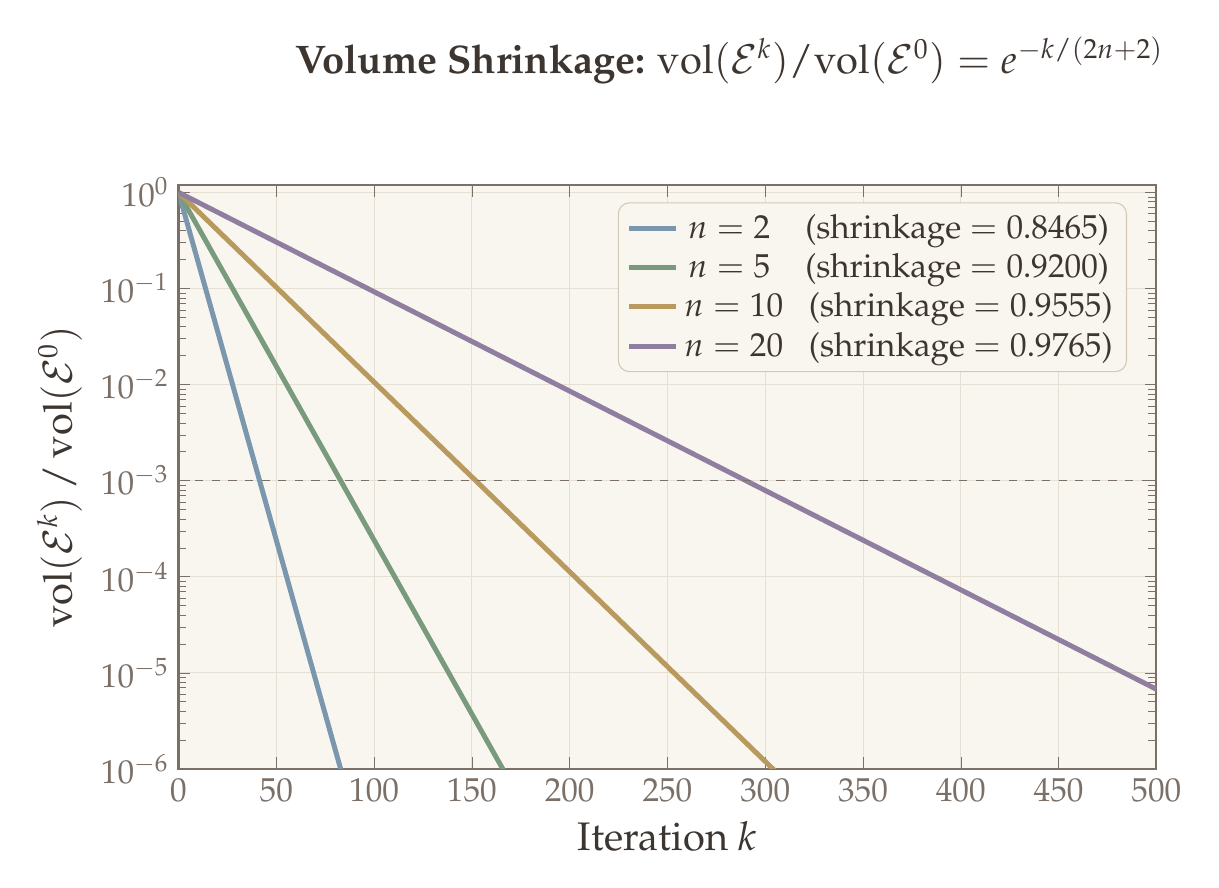
\begin{tikzpicture}

\begin{axis}[
    width=14cm,
    height=9cm,
    axis background/.style={fill=cream},
    xlabel={Iteration $k$},
    ylabel={$\mathrm{vol}(\mathcal{E}^k) \,/\, \mathrm{vol}(\mathcal{E}^0)$},
    xlabel style={font=\Large, text=dkbrown},
    ylabel style={font=\Large, text=dkbrown},
    xmin=0, xmax=500,
    ymin=1e-6, ymax=1.2,
    ymode=log,
    grid=major,
    grid style={border!60, line width=0.3pt},
    tick label style={font=\large, text=wmgray},
    legend style={
      at={(0.97,0.97)},
      anchor=north east,
      font=\large,
      draw=border,
      fill=cream,
      rounded corners=4pt,
      text=dkbrown,
    },
    every axis plot/.append style={line width=1.8pt, no marks},
    axis line style={wmgray, line width=0.8pt},
    tick style={wmgray},
  ]

  % n = 2: shrinkage per step = exp(-1/(2*3)) = exp(-1/6) ≈ 0.8465
  % After k steps: (0.8465)^k
  \addplot[stblue, domain=0:500, samples=100]
    {exp(-x/6)};
  \addlegendentry{$n = 2$ \;\; (shrinkage $= 0.8465$)}

  % n = 5: shrinkage per step = exp(-1/(2*6)) = exp(-1/12) ≈ 0.9200
  \addplot[sage, domain=0:500, samples=100]
    {exp(-x/12)};
  \addlegendentry{$n = 5$ \;\; (shrinkage $= 0.9200$)}

  % n = 10: shrinkage per step = exp(-1/(2*11)) = exp(-1/22) ≈ 0.9555
  \addplot[rwgold, domain=0:500, samples=100]
    {exp(-x/22)};
  \addlegendentry{$n = 10$ \; (shrinkage $= 0.9555$)}

  % n = 20: shrinkage per step = exp(-1/(2*21)) = exp(-1/42) ≈ 0.9765
  \addplot[lavender, domain=0:500, samples=100]
    {exp(-x/42)};
  \addlegendentry{$n = 20$ \; (shrinkage $= 0.9765$)}

  % Reference line at 10^{-3}
  \addplot[wmgray, dashed, line width=0.6pt, domain=0:500, samples=2]
    {1e-3};
  \node[font=\normalsize, text=wmgray, anchor=west] at (axis cs:510,1e-3) {};

\end{axis}

% Title
\node[font=\Large\bfseries, text=dkbrown] at (7,9.0)
  {Volume Shrinkage: $\mathrm{vol}(\mathcal{E}^k)/\mathrm{vol}(\mathcal{E}^0) = e^{-k/(2n+2)}$};

\end{tikzpicture}
\end{document}
